%!TEX root = proj_report_outline.tex
\chapter{Evaluation}

\section{Functionality}

\subsection{User Stories}
To evaluate whether the requirements D1, D2.1 and D2.2 have been fulfilled, the system's behaviour was tested in regards to each of these requirements. 
Requirement D1's user stories specify the ability to post Pitch Cards, make suggestions on Pitch Points, accept/reject Pitch Points, comment on Pitch Points, comment on suggestions and mark Pitch Cards as completed/active. 

Requirement D2.1's user stories specify the ability to scope entities such as Pitch Cards, Suggestions, and one's identity such that unintended viewers are avoided. To ensure the completeness of these scope tests these user stories were derived from the following behaviour matrix:

\begin{figure}[ht]
    \centering
    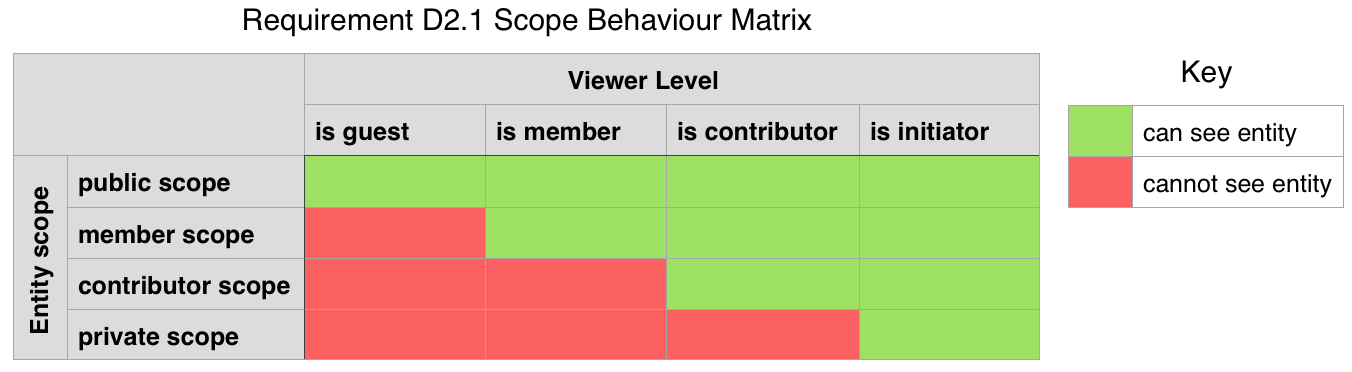
\includegraphics[width=1\textwidth]{scope_matrix}
    \caption{The scope matrix which illustrates the relationship between user level and entity scope in regards to viewing the entity.}
    \label{fig:architecturescope_matrix_evaluation}
\end{figure}


Requirement D2.2's user stories specify that users who have viewed a Pitch Card are able to be seen as a ``viewer'' by the initiator.

Given that these user stories are verified as working by \textit{TB3} it is concluded that requirements D1, D2.1 and D2.2 have been fulfilled.

\subsection{Deployed Prototype}
At the time of writing, the prototype has been successfully been deployed to Callaghan Innovation and is ready for use. Unfortunately use of the prototype by Callaghan Innovation has not yet fully commenced. Without substantial activity to analyse this component of the evaluation was unable to be completed. It is expected that the access code will be distributed by the Callaghan Innovation stakeholders to the wider organisation in the coming weeks.

\section{Performance}

\subsection{Nielsen's Response Time Thresholds}

\subsection{Test 1 - User Size}

\subsection{Test 2 - Overhead of Threshold Scheme Security}

\subsection{Test 3 - Overhead of Secret Keeper Diversity}

\subsection{Discussion}

A limitation of the experiment described in Section \ref{SS:performance} is that it is only semi-globally distributed. Two servers hosted on AWS (located in Oregon, USA) and two servers hosted by Callaghan Innovation in Wellington provide an uncommon network topology. The Secret Sharing Service with the ``3, 4'' threshold scheme means that on each database query at least one request will be sent to one of the AWS instances. This impacts the performance results due to the latency incurred. For performance results it would have been better to have all servers hosted within New Zealand. However, security and disaster recovery considerations motivated the move to embrace a more geographically distributed network.

The disadvantage of unconditionally secure secret sharing schemes is that the storage and transmission of the shares requires an amount of storage and bandwidth resources equivalent to the size of the secret times the number of shares. If the size of the secret were significant, say 1 GB, and the number of shares were 10, then 10 GB of data must be stored by the shareholders
